\documentclass[12pt]{article}

%%%%%%%%%%%%%%%%%%%%%%%%%%%%%%%%%%%%%%%%%%%%%%%%%%%%%%%%%%%%%%%%%%%%%%%%%%%%%%%%
%                           Package preset for homework
%%%%%%%%%%%%%%%%%%%%%%%%%%%%%%%%%%%%%%%%%%%%%%%%%%%%%%%%%%%%%%%%%%%%%%%%%%%%%%%%
% Miscellaneous
\usepackage[margin=1in]{geometry}
\usepackage[utf8]{inputenc}
\usepackage{indentfirst}
\usepackage{blindtext}
\usepackage{graphicx}
\usepackage{xr-hyper}
\usepackage{hyperref}
\usepackage{enumitem}
\usepackage{color}
\usepackage{float}
% Math
\usepackage{latexsym}
\usepackage{amsfonts}
\usepackage{amssymb}
\usepackage{amsmath}
\usepackage{commath}
\usepackage{amsthm}
\usepackage{bbold}
\usepackage{bm}
% Physics
\usepackage{physics}
\usepackage{siunitx}
% Code typesetting
\usepackage{listings}
% Citation
\usepackage[authoryear]{natbib}
\usepackage{appendix}
\usepackage[capitalize]{cleveref}
% Title & name
\title{Homework}
\author{Tien Vo}
\date{\today}


%%%%%%%%%%%%%%%%%%%%%%%%%%%%%%%%%%%%%%%%%%%%%%%%%%%%%%%%%%%%%%%%%%%%%%%%%%%%%%%%
%                   User-defined commands and environments
%%%%%%%%%%%%%%%%%%%%%%%%%%%%%%%%%%%%%%%%%%%%%%%%%%%%%%%%%%%%%%%%%%%%%%%%%%%%%%%%
%%% Misc
\sisetup{load-configurations=abbreviations}
\newcommand{\due}[1]{\date{Due: #1}}
\newcommand{\hint}{\textit{Hint}}
\let\oldt\t
\renewcommand{\t}[1]{\text{#1}}

%%% Bold sets & abbrv
\newcommand{\N}{\mathbb{N}}
\newcommand{\Z}{\mathbb{Z}}
\newcommand{\R}{\mathbb{R}}
\newcommand{\Q}{\mathbb{Q}}
\let\oldP\P
\renewcommand{\P}{\mathbb{P}}
\newcommand{\LL}{\mathcal{L}}
\newcommand{\FF}{\mathcal{F}}
\newcommand{\HH}{\mathcal{H}}
\newcommand{\NN}{\mathcal{N}}
\newcommand{\ZZ}{\mathcal{Z}}
\newcommand{\RN}[1]{\textup{\uppercase\expandafter{\romannumeral#1}}}
\newcommand{\ua}{\uparrow}
\newcommand{\da}{\downarrow}

%%% Unit vectors
\newcommand{\xhat}{\vb{\hat{x}}}
\newcommand{\yhat}{\vb{\hat{y}}}
\newcommand{\zhat}{\vb{\hat{z}}}
\newcommand{\nhat}{\vb{\hat{n}}}
\newcommand{\rhat}{\vb{\hat{r}}}
\newcommand{\phihat}{\bm{\hat{\phi}}}
\newcommand{\thetahat}{\bm{\hat{\theta}}}

%%% Other math stuff
\providecommand{\units}[1]{\,\ensuremath{\mathrm{#1}}\xspace}
% Set new style for problem
\newtheoremstyle{problemstyle}  % <name>
        {10pt}                   % <space above>
        {10pt}                   % <space below>
        {\normalfont}           % <body font>
        {}                      % <indent amount}
        {\bfseries\itshape}     % <theorem head font>
        {\normalfont\bfseries:} % <punctuation after theorem head>
        {.5em}                  % <space after theorem head>
        {}                      % <theorem head spec (can be left empty, 
                                % meaning `normal')>

% Set problem environment
\theoremstyle{problemstyle}
\newtheorem{problemenv}{Problem}[section]
\newenvironment{problem}[1]{%
  \renewcommand\theproblemenv{#1}%
  \problemenv
}{\endproblemenv}
% Set lemma environment
\newenvironment{lemma}[2][Lemma]{\begin{trivlist}
\item[\hskip \labelsep {\bfseries #1}\hskip \labelsep {\bfseries #2.}]}{\end{trivlist}}
% Set solution environment
\newenvironment{solution}{
    \begin{proof}[Solution]$ $\par\nobreak\ignorespaces
}{\end{proof}}
\numberwithin{equation}{problemenv}

%%% Page format
\setlength{\parindent}{0.5cm}
\setlength{\oddsidemargin}{0in}
\setlength{\textwidth}{6.5in}
\setlength{\textheight}{8.8in}
\setlength{\topmargin}{0in}
\setlength{\headheight}{18pt}

%%% Code environments
\definecolor{dkgreen}{rgb}{0,0.6,0}
\definecolor{gray}{rgb}{0.5,0.5,0.5}
\definecolor{mauve}{rgb}{0.58,0,0.82}
\lstset{frame=tb,
  language=Python,
  aboveskip=3mm,
  belowskip=3mm,
  showstringspaces=false,
  columns=flexible,
  basicstyle={\small\ttfamily},
  numbers=none,
  numberstyle=\tiny\color{gray},
  keywordstyle=\color{blue},
  commentstyle=\color{dkgreen},
  stringstyle=\color{mauve},
  breaklines=true,
  breakatwhitespace=true,
  tabsize=4
}
\lstset{
  language=Mathematica,
  numbers=left,
  numberstyle=\tiny\color{gray},
  numbersep=5pt,
  breaklines=true,
  captionpos={t},
  frame={lines},
  rulecolor=\color{black},
  framerule=0.5pt,
  columns=flexible,
  tabsize=2
}


\title{Homework 2: Phys 5210 (Fall 2021)}

\begin{document}


\maketitle

%%%%%%%%%%%%%%%%%%%%%%%%%%%%%%%%%%%%%%%%%%%%%%%%%%%%%%%%%%%%%%%%%%%%%%%%%%%%%%%%
\begin{problem}{1}

The period of oscillations of a pendulum (a point mass $m$ connected to a
massless rod of length $l$ which in turn is connected to the ceiling) is equal
to $T=2\pi\sqrt{l/g}$ where $g$ is free fall acceleration if the amplitude of
the oscillations of the pendulum is very small. Find the first correction to
this due to the finite magnitude of the oscillations assuming that it is
small.

\textit{Hint}: You will encounter an integral which mathematica does not handle
very well. Please substitute $\cos\theta=1-2\sin^2(\theta/2)$ into the integral
before attempting to do any of the integrals. The answer will be expressed in
terms of the elliptic integral of the first kind, and mathematica should handle
those. Expand the answer in powers of the amplitude using mathematica (or the
handbook of mathematical functions).

\begin{solution}
    \begin{center}
        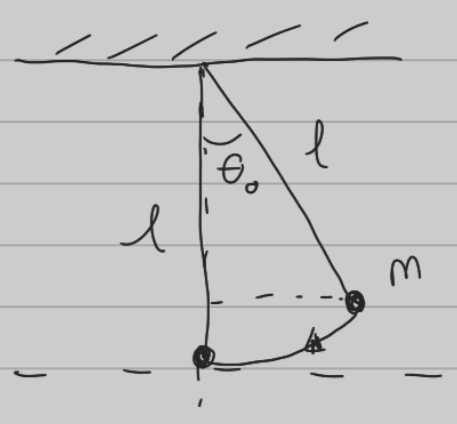
\includegraphics[width=0.5\textwidth]{hw2_p1.jpg} 
    \end{center}
    Let the potential be zero at the lowest point of the pendulum. Then the
    energy of the system is
    \begin{equation}
        E=\frac12ml^2\dot{\theta}^2+mgl(1-\cos\theta)
    \end{equation}
    Since the potential is time independent, the energy is conserved. We can 
    then write from the initial conditions
    $\theta(t=0)=\theta_0$ and $\dot{\theta}(t=0)=0$
    \begin{equation}
        \frac12ml^2\dot{\theta}^2+mgl(1-\cos\theta)=mgl(1-\cos\theta_0)
    \end{equation}
    Inverting, we arrive at a differential equation
    \begin{equation}
        \frac{d\theta}{dt}
        =\sqrt{\frac{2g}{l}}\sqrt{\cos\theta-\cos\theta_0}
        =2\sqrt{\frac{g}{l}}
        \sqrt{\sin^2\qty(\frac{\theta_0}{2})-\sin^2\qty(\frac{\theta}{2})} 
    \end{equation}
    A period of the pendulum consists of these four phases: (1) $\theta_0\to0$,
    (2) $0\to-\theta_0$, (3) $-\theta_0\to0$, and (4) $0\to\theta_0$. By
    symmetry, $T=4t_{0\to\theta_0}$. Now we integrate
    \begin{align}
        t_{0\to\theta_0}&=\frac12\sqrt{\frac{l}{g}}\int_0^{\theta_0}d\theta
        \qty[\sin^2\qty(\frac{\theta_0}{2})-\sin^2\qty(\frac{\theta}{2})]^{-1/2}
        \notag\\
                        &=\sqrt{\frac{l}{g}}\int_0^1\frac{du}{\sqrt{1-u^2}\sqrt{1-k^2u^2}}\tag{$k=\sin(\theta_0/2),ku=\sin\qty(\theta/2)$}\\
                        &=\sqrt{\frac{l}{g}}K(k^2)
    \end{align}
    where $K$ is the complete elliptic integral of the first kind. By the
    designated transformation $\theta\mapsto u$, we have
    $2kdu=\sqrt{1-\sin^2(\theta/2)}d\theta=\sqrt{1-k^2u^2}d\theta$. Substituting
    into the first equality, we get the second equality. Now, we can expand $K$
    in small $\theta$
    \begin{equation}
        t_{0\to\theta_0}=\sqrt{\frac{l}{g}}\qty[\frac\pi2+\frac\pi{32}\theta_0^2+\order{\theta_0^4}]
    \end{equation}
    It then follow that the period $T$ is
    \begin{equation}
        T=4t_{0\to\theta_0}=2\pi\sqrt{\frac{l}{g}}\qty[1+\frac1{16}\theta_0^2+\order{\theta_0^4}]
    \end{equation}
    So the next order correction to the period is $T_1=(\theta_0^2/16)T_0$
    where $T_0=2\pi\sqrt{l/g}$ is the lowest order period of the pendulum.
\end{solution}

\end{problem}
%%%%%%%%%%%%%%%%%%%%%%%%%%%%%%%%%%%%%%%%%%%%%%%%%%%%%%%%%%%%%%%%%%%%%%%%%%%%%%%%
\begin{problem}{2}
A very thin vertical wheel (think of a bicycle wheel with weightless spokes) of
radius $R$ and mass $m$ has a pebble of mass $M$ permanently attached to its
rim. A wheel is set up vertically with the pebble at the top point of the wheel,
and given an infintesimally weak push which sets it rolling without slipping by
gravity pulling the pebble down. How heavy should the pebble be so that at some
moment in time the wheel would go airborne?

Useful information: kinetic energy of this kind of a wheel is equal to
$mv^2/2+mR^2\omega^2/2$ where $v$ is its velocity (velocity of its center) and
$\omega$ is its angular velocity.

\begin{solution}
    \begin{center}
        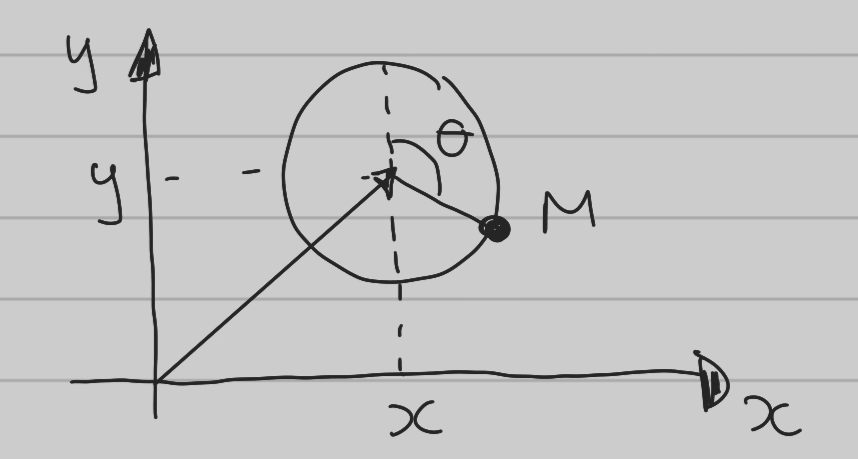
\includegraphics[width=0.5\textwidth]{hw2_p2.jpg} 
    \end{center} 

    Define a coordinate system as above. The center of the wheel is $(x,y)$ and
    the position of the pebble is
    \begin{equation}
        \begin{cases}
            x_M&=x+R\sin\theta\\
            y_M&=y+R\cos\theta
        \end{cases} 
        \Rightarrow
        \begin{cases}
            \dot{x_M}&=\dot{x}+R\cos\theta\dot\theta\\
            \dot{y_M}&=\dot{y}-R\sin\theta\dot\theta
        \end{cases}
    \end{equation}
    Then the kinetic energy $T_M$ and the potential energy $V_M$ of the pebble
    is
    \begin{subequations}\label{p2:pebble}
    \begin{align}
        T_M&=\frac12M\qty(\dot{x_M}^2+\dot{y_M}^2) 
        +\frac12M\qty[\dot{x}^2+\dot{y}^2+R^2\dot\theta^2
        +2R(\dot{x}\cos\theta-\dot{y}\sin\theta)\dot\theta
        ]\\
        V_M&=Mgy_M=Mg(y+R\cos\theta)
    \end{align} 
    \end{subequations}
    Similarly, the kinetic energy $T_W$ and the potential energy $V_W$ of the 
    wheel is
    \begin{subequations}\label{p2:wheel}
    \begin{align}
        T_W&=\frac12m\qty(\dot{x}^2+\dot{y}^2+R^2\dot\theta^2)\\
        V_W&=mgy       
    \end{align} 
    \end{subequations}
    If the wheel rolls without slipping, then it must also follow that
    $\dot{x}=R\dot\theta$. Then we can write the total energy from
    \eqref{p2:pebble} and \eqref{p2:wheel} as
    \begin{align}
        E&=\frac12\qty(M+m)\qty(2R^2\dot\theta^2+\dot{y}^2)+MR^2\cos\theta\dot\theta^2-MR\sin\theta\dot{y}\dot\theta+(M+m)gy+MgR\cos\theta\notag\\
         &=(2M+m)gR
    \end{align}
    where the last equality comes from energy conservation. The initial
    conditions are $y=R$, $\theta=0$, and $\dot\theta=\dot{y}=0$. Imposing the
    constraint $f(y)=y-R=0$ that the wheel touches the ground, then we can solve
    for
    \begin{equation}\label{p2:td}
        R\dot\theta^2=\frac{M(1-\cos\theta)}{m+M+M\cos\theta}g
    \end{equation}

    Now, the Lagrange function with the constraint $f$ and the Lagrange
    multiplier $\lambda$ is
    \begin{equation}
        \LL=\frac12(M+m)\qty(2R^2\dot\theta^2+\dot{y}^2)+MR^2\cos\theta\dot\theta^2-MR\sin\theta\dot{y}\dot\theta-(M+m)gy-MgR\cos\theta-\lambda(y-R) 
    \end{equation}
    Using the Euler-Lagrange equation for $\theta$,
    \begin{align}
        \frac{\partial\LL}{\partial\theta}
        &=-MR^2\sin\theta\dot\theta^2-MR\cos\theta\dot{y}\dot\theta+MgR\sin\theta\notag\\
        &=\frac{d}{dt}\frac{\partial\LL}{\partial\dot\theta}\notag\\
        &=-2M\sin\theta
        R^2\dot\theta^2+2(m+M+M\cos\theta)R^2\ddot\theta-MR\cos\theta\dot{y}\dot\theta-MR\sin\theta\ddot{y}
    \end{align}
    Since $\dot{y}=\ddot{y}=0$ due to $f$, we can write
    \begin{equation}\label{p2:tdd}
        R\ddot\theta=\frac{M\sin\theta}{2(m+M+M\cos\theta)}\qty(R\dot\theta^2+g) 
    \end{equation}
    
    The Euler-Lagrange equation for $y$ gives
    \begin{equation}
        -(M+m)g-\lambda=(M+m)\ddot{y}-MR\cos\theta\dot\theta^2-MR\sin\theta\ddot\theta 
    \end{equation}
    Note that $-\lambda$ plays the role of the normal force. So if
    $\lambda\geq0$, the normal force is negative and the wheel becomes airborne.
    Using the constraint $f$, \eqref{p2:td}, and \eqref{p2:tdd}, we can solve
    for $\lambda$ (see Mathematica code at the end of the solution)
    \begin{align}
        \lambda&=\frac{g}{2}\qty[
            \frac{M^2\sin^2\theta(m+2M)}{(m+M+M\cos\theta)^2}
            +\frac{2M^2(1-\cos\theta)\cos\theta}{m+M+M\cos\theta}-2(M+m)
        ]\notag\\
       &=\frac{Mg}{2}\qty[
            \frac{\sin^2\theta(\xi+2)}{(\xi+1+\cos\theta)^2}
            +\frac{2(1-\cos\theta)\cos\theta}{\xi+1+\cos\theta}
            -2(1+\xi)
       ]
    \end{align}
    where $\xi=m/M$ is the wheel-pebble mass ratio. The heatmap below shows the
    value for $\lambda$ in terms of $\xi$ and $\theta$ where $\lambda<0$ is
    plotted in white and $\lambda\geq0$ is colorred according to the colorbar.
    \begin{center}
        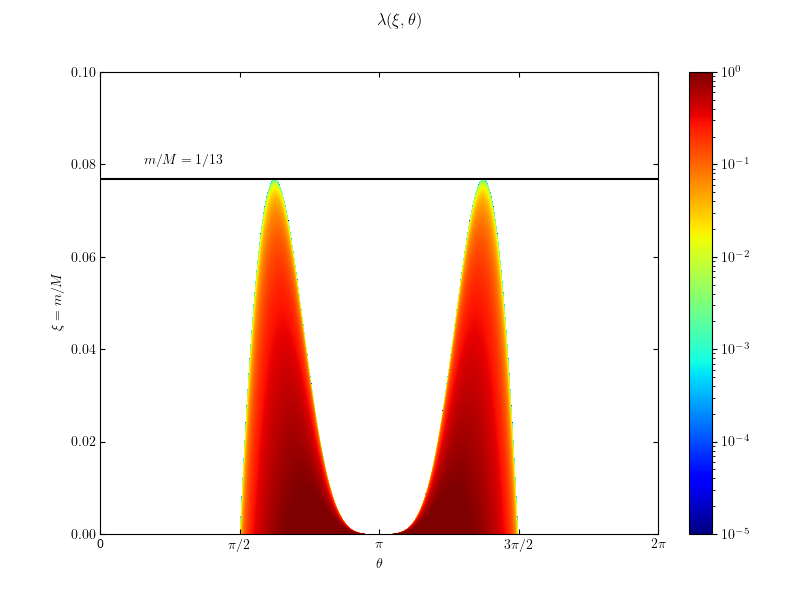
\includegraphics[width=0.8\textwidth]{fig.png} 
    \end{center}

    First note that the angle at which $\lambda$ becomes positive is symmetric
    over $\theta=\pi$. This is because the initial perturbation in either
    direction (in $x$) would lead to similar results. Now, if the wheel rolls
    forward in $x$, it goes airborne for $\theta\geq\pi/2$ if the mass of the
    pebble is dominant ($\xi\ll1$). For $\pi/2\leq\theta\leq\pi$, the boundary
    between colorred and white region shows the limit for $\xi$ at which the
    wheel goes airborne. For example, the largest limit is $\xi<1/13$ as
    indicated in the figure. This means the pebble has to be at least 13 times 
    the mass of the wheel for the system to go airborne at
    $\theta\approx113^\circ$. For lower limits of $\xi$, $M$ has to be even
    larger.

\begin{center}
    \textit{Mathematica code}  
\end{center}
\begin{lstlisting}[startnumber=1]
rthetad2 = (M (1 - Cos[\[Theta]]) g)/(m + M + M Cos[\[Theta]]);
rthetadd = (M Sin[\[Theta]] (rthetad2 + g))/(2 (m + M + M Cos[\[Theta]]));
Simplify[-(M + m) g + M Cos[\[Theta]] rthetad2 + M Sin[\[Theta]] rthetadd] 
\end{lstlisting}
\end{solution}
\end{problem}
%%%%%%%%%%%%%%%%%%%%%%%%%%%%%%%%%%%%%%%%%%%%%%%%%%%%%%%%%%%%%%%%%%%%%%%%%%%%%%%%

\end{document}
